\documentclass{article}
\usepackage{amsmath}
\usepackage{amssymb}
\usepackage{pgfplots, capt-of}
\pgfplotsset{width=10cm,compat=1.9}
\title{Matrix Rotations}
\author{James Blackburn}
\date{January 2022}
\begin{document}
\maketitle
\section{Using the angle between two vectors}
First of all, we can define the 2x2 matrix inversion in the variable $\boldsymbol{R}$ as:
\begin{gather} 
\text{Where }\theta \text{ is the anti-clockwise angle of rotation.} \\
\boldsymbol{R}  = \begin{bmatrix}\cos \theta & -\sin \theta \\ \sin \theta & \cos \theta \end{bmatrix} 
\end{gather} 
The general form of vectors is:

\begin{gather} 
\vec{v} = \begin{bmatrix}x  \\ y \end{bmatrix} 
\end{gather} 
Now let's take the identity matrix:

\begin{gather} 
\boldsymbol{I} = \begin{bmatrix}1 & 0 \\ 0 & 1 \end{bmatrix} 
\end{gather} 
Now, let's take the vector of the positive x-axis and the positive y-axis:

\begin{gather} 
\vec{a} = \begin{bmatrix}1  \\ 0 \end{bmatrix} \\
\vec{b} = \begin{bmatrix}0  \\ 1 \end{bmatrix} 
\end{gather} 
And rotate this by the matrix $\boldsymbol{R}$:

\begin{gather} 
\vec{c} = \begin{bmatrix}\cos \theta & -\sin \theta \\ \sin \theta & \cos \theta \end{bmatrix}  \begin{bmatrix}1  \\ 0 \end{bmatrix} =  \begin{bmatrix}\cos \theta  \\ \sin \theta \end{bmatrix} \\
\vec{d} = \begin{bmatrix}\cos \theta & -\sin \theta \\ \sin \theta & \cos \theta \end{bmatrix}  \begin{bmatrix}0 \\ 1 \end{bmatrix} =  \begin{bmatrix}-\sin \theta  \\ \cos \theta \end{bmatrix}
\end{gather} 

Using this function, we can give evidence of the dot product between two vectors. 
\\The dot product is defined as such (where $a$ and $b$ are random variables):

\begin{gather*} 
\cos \theta = \frac{x_a \times x_b+y_a \times y_b}{\left \lvert a \right \rvert \times \left \lvert b \right \rvert}
\end{gather*} 
This can be re-arranged to find $\theta$ (theta):
\begin{gather*} 
\theta = \cos^{-1}\left (  \frac{x_a \times x_b+y_a \times y_b}{\lvert \vec{a} \rvert \times \lvert \vec{b}  \rvert} \right )\label{eq:dotproduct}
\end{gather*} 
Now let's find the rotation between $\vec{a}$ \& $\vec{c}$ and $\vec{b}$ \& $\vec{d}$:
\begin{gather}
\begin{split}
\theta_1 = \cos^{-1}\left (  \frac{1 \times \cos \theta + 0 \times \sin \theta}{\sqrt{1^2 + 0^2} \times \sqrt{(\cos \theta)^2 + (\sin \theta)^2}} \right ) \\
=  \cos^{-1}\left ( \frac{\cos \theta}{\sqrt{1^2 + 0^2} \times \sqrt{\cos^2 \theta + \sin^2 \theta}}   \right ) \\
=  \cos^{-1}\left ( \frac{\cos \theta}{1 \times 1}   \right ) \\
=  \cos^{-1}\left ( \cos \theta  \right ) \\
= \theta
\end{split} \\
\begin{split}
\theta_2 = \cos^{-1}\left (  \frac{0 \times -\sin \theta + 1 \times \cos \theta}{\sqrt{0^2 + 1^2} \times \sqrt{(-\sin \theta)^2 + (\cos \theta)^2}} \right ) \\
= \cos^{-1}\left ( \frac{\cos \theta}{\sqrt{0^2 + 1^2} \times \sqrt{\sin^2 \theta + \cos^2 \theta}}   \right ) \\
=  \cos^{-1}\left ( \frac{\cos \theta}{1 \times 1}   \right ) \\
=  \cos^{-1}\left ( \cos \theta  \right ) \\
= \theta
\end{split}
\end{gather}
Therefore, we have proved that the rotation matrix $\boldsymbol{R}$ rotates a vector by the angle $\theta$.

\begin{minipage}{\textwidth}
Alongside this proof, we have also managed to prove another fact:
Given any 2d matrix, one can instantly tell if it's a rotation matrix by the following test:

\begin{gather}
\boldsymbol{A} =  \begin{bmatrix}a & b \\ c & d \end{bmatrix} \\
\sqrt{a^2+c^2} = 1 \\
\sqrt{b^2+d^2} = 1 
\end{gather}
\begin{gather*}
\text{Because:}
\end{gather*}
\begin{gather}
\sqrt{cos^2 \theta+sin^2 \theta} = 1 \\
\sqrt{sin^2 \theta + cos^2 \theta} = 1 
\end{gather}
\end{minipage}	

\section{Clockwise or anti-clockwise}

Considering that a rotation is always going to be in the range $0 \leq \theta \leq 360$ and considering the 3 functions we use in the matrix $\boldsymbol{R}$ are $\sin \theta$, $\cos \theta$ and $-\sin \theta$, we can plot these functions onto a graph:

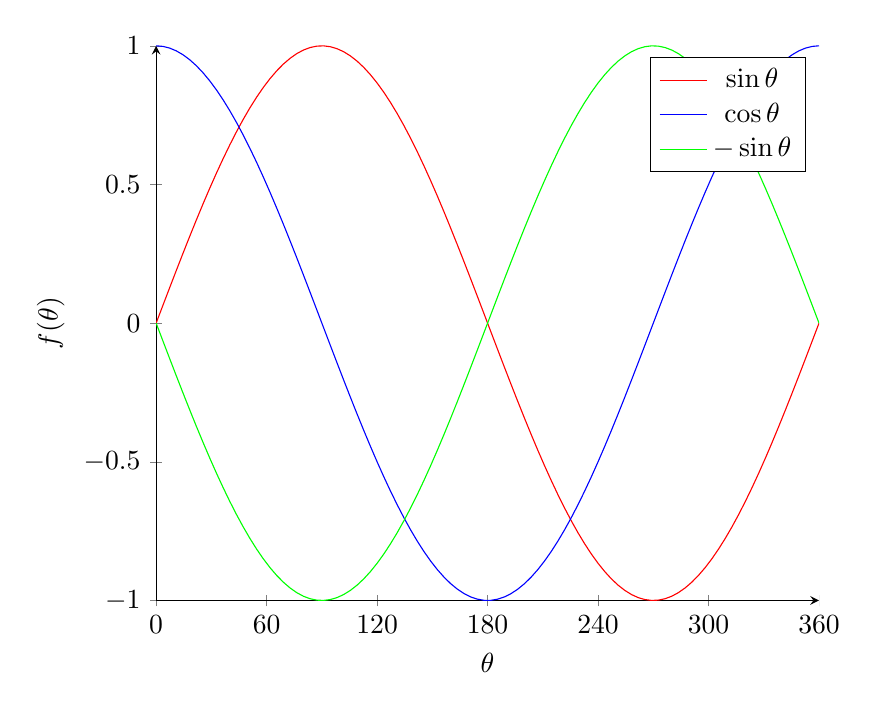
\begin{tikzpicture}
\begin{axis}[
    axis lines = left,
    xlabel = $\theta$,
    ylabel = {$f(\theta)$},
    xtick={0,60,120,180,240, 300, 360},
]
\addplot [
    domain=0:360, 
    samples=100, 
    color=red,
]
{sin x};
\addlegendentry{\(\sin \theta\)}
\addplot [
    domain=0:360, 
    samples=100, 
    color=blue,
    ]
    {cos x};
\addlegendentry{\(\cos \theta \)}
\addplot [
    domain=0:360, 
    samples=100, 
    color=green,
]
{-sin x};
\addlegendentry{\(-\sin \theta\)}
\end{axis}
\end{tikzpicture}
\captionof{figure}{Domain: $0 \leq \theta \leq 360$, Range: $-1 \leq f(\theta) \leq 1$}

\begin{minipage}{\textwidth}
Now, let's consider what an anti-clockwise and clockwise rotation actually is. Because we know that the matrix $\boldsymbol{R}$ gives an anti-clockwise rotation, we know that $0 \leq \theta \leq 180$ is anti-clockwise, hence $180 \leq \theta \leq 360$ is clockwise.
\end{minipage}	

Let's zoom in to the $\cos \theta$ graph:

\begin{tikzpicture}
\begin{axis}[
    axis lines = left,
    xlabel = \(\theta\),
    ylabel = {\(f(\theta)\)},
    xtick={0,60,120,180,240, 300, 360},
]
\addplot [
    domain=0:180, 
    samples=100, 
    color=blue,
    ]
    {cos x};
\addlegendentry{\(\cos \theta \) acw}
\addplot [
    domain=180:360, 
    samples=100, 
    color=green,
    ]
    {cos x};
\addlegendentry{\(\cos \theta \) cw}
\addplot coordinates {(180,-1)(180,1)};
\end{axis}
\end{tikzpicture}
\captionof{figure}{Domain: $0 \leq \theta \leq 360$, Range: $-1 \leq f(\theta) \leq 1$}


Can you see how it doesn't matter whether the rotation is clockwise or anti-clockwise? It is negative or positive in either of these cases. This means we can forget about the cosine graph for now! Let's move onto $\sin \theta$ and $-\sin \theta$!

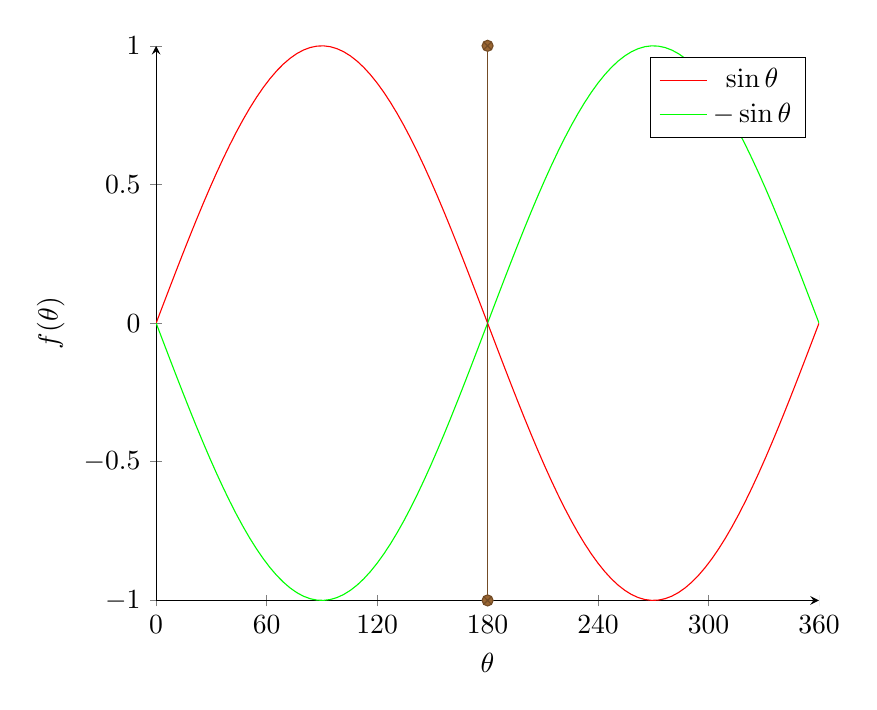
\begin{tikzpicture}
\begin{axis}[
    axis lines = left,
    xlabel = \(\theta\),
    ylabel = {\(f(\theta)\)},
    xtick={0,60,120,180,240, 300, 360},
]
\addplot [
    domain=0:360, 
    samples=100, 
    color=red,
]
{sin x};
\addlegendentry{\(\sin \theta\)}
\addplot [
    domain=0:360, 
    samples=100, 
    color=green,
]
{-sin x};
\addlegendentry{\(-\sin \theta\)}
\addplot coordinates {(180,-1)(180,1)};
\end{axis}
\end{tikzpicture}
\captionof{figure}{Domain: $0 \leq \theta \leq 360$, Range: $-1 \leq f(\theta) \leq 1$}

Can you see how the graphs converge at $180^o$? This means that in the domain $0 \leq \theta \leq 180$ (anti-clockwise), $0 \leq \sin \theta \leq 1$ and $-1 \leq -\sin \theta \leq 0$. Hence, for the domain $180 \leq \theta \leq 360$ (clockwise), $-1 \leq \sin \theta \leq 0$ and $0 \leq -\sin \theta \leq -1$.

But what does this actually mean for a mathematician? Well, it means, given the following rotation matrix:

\[\boldsymbol{B} =  \begin{bmatrix}\frac{1}{2} & -\frac{\sqrt{3}}{2} \\[6pt] \frac{\sqrt{3}}{2} & \frac{1}{2} \end{bmatrix} \]

We can see that $\boldsymbol{B}_{12}$  (the top right corner) is negative. Therefore, it is an anticlockwise rotation!

Now let's take another matrix $\boldsymbol{C}$:

\[\boldsymbol{C} =  \begin{bmatrix}\frac{1}{\sqrt{2}} & \frac{1}{\sqrt{2}} \\[6pt] -\frac{1}{\sqrt{2}} & \frac{1}{\sqrt{2}} \end{bmatrix} \]

We can see that $\boldsymbol{C}_{21}$  (the bottom left corner) is negative. Therefore, it is a clockwise rotation!
%Defining the two vectors $\vec{a}$, $\vec{b}$:
%
%
%\begin{gather} 
%\vec{a} = \begin{bmatrix}cos \theta  \\ sin \theta \end{bmatrix} \\
%\vec{b} = \begin{bmatrix}-sin \theta  \\ cos \theta \end{bmatrix}
%\end{gather}  
%
%\begin{minipage}{\textwidth}
%Substituting these values into the formula above \eqref{eq:dotproduct} gives:
%
%\begin{gather} 
%\theta = \cos^{-1}\left (  \frac{\cos \theta \times -\sin \theta + \sin \theta \times \cos \theta}{\sqrt{(\cos \theta)^2 + (\sin \theta)^2} \times \sqrt{(-\sin \theta)^2 + (\cos \theta)^2}} \right )
%\end{gather} 
%\end{minipage}
%
%Factoring out $\cos \theta$ gives:
%
%\begin{gather} 
%\theta = \cos^{-1}\left (  \frac{\cos \theta ( -\sin \theta + \sin \theta)}{\sqrt{(\cos \theta)^2 + (\sin \theta)^2} \times \sqrt{(-\sin \theta)^2 + (\cos \theta)^2}} \right )
%\end{gather} 


\end{document}